\documentclass[12pt,a4paper]{article}

% ─── Page Layout ───────────────────────────────────────────────────────────────
\usepackage[a4paper, margin=0.8in, headheight=14pt]{geometry}

% ─── Fonts (XeLaTeX) ───────────────────────────────────────────────────────────
\usepackage{fontspec}
\usepackage{unicode-math}
\setmainfont{TeX Gyre Pagella}
\setmonofont[Scale=0.88]{TeX Gyre Cursor}
\setmathfont{Latin Modern Math}

% ─── Packages ──────────────────────────────────────────────────────────────────
\usepackage{xcolor}
\usepackage{colortbl}
\usepackage{titlesec}
\usepackage{enumitem}
\usepackage{tabularx}
\usepackage{booktabs}
\usepackage{array}
\usepackage{amsmath}
\usepackage{tikz}
\usetikzlibrary{shapes.geometric, arrows.meta, positioning, calc, fit, decorations.pathreplacing}
\usepackage{tcolorbox}
\tcbuselibrary{skins, breakable}
\usepackage{hyperref}
\usepackage{fancyhdr}
\usepackage{graphicx}
\usepackage{microtype}
\hyphenpenalty=10000
\exhyphenpenalty=10000
\sloppy
\usepackage{caption}
\usepackage{setspace}
\usepackage{multirow}
\usepackage{tocloft}

% ─── Q&A helper ────────────────────────────────────────────────────────────────
\newcommand{\Q}[1]{\textbf{#1}\par\noindent\ignorespaces}

% ─── Colour Palette ────────────────────────────────────────────────────────────
\definecolor{myred}{RGB}{196,30,58}
\definecolor{mydark}{RGB}{30,30,50}
\definecolor{mygreen}{RGB}{14,120,80}
\definecolor{myteal}{RGB}{0,130,140}
\definecolor{myamber}{RGB}{180,100,0}
\definecolor{mypurple}{RGB}{100,30,160}
\definecolor{mygray}{RGB}{246,247,249}
\definecolor{mgframe}{RGB}{180,185,200}
\definecolor{watermark}{RGB}{145,150,170}
\definecolor{hdrred}{RGB}{250,232,235}
\definecolor{hdrgreen}{RGB}{220,244,233}
\definecolor{hdrteal}{RGB}{220,242,244}
\definecolor{hdramber}{RGB}{253,242,215}
\definecolor{hdrpurple}{RGB}{238,228,255}
\definecolor{hdrgray}{RGB}{238,240,245}
\definecolor{rowalt}{RGB}{250,251,253}

% ─── Section Formatting ────────────────────────────────────────────────────────
\titleformat{\section}
  {\large\bfseries\color{myred}}{\thesection.}{0.5em}{}
  [\vspace{1pt}{\color{myred}\rule{\linewidth}{0.8pt}}]
\titleformat{\subsection}
  {\normalsize\bfseries\color{myteal}}{\thesubsection}{0.5em}{}
\titlespacing*{\section}{0pt}{18pt}{7pt}
\titlespacing*{\subsection}{0pt}{11pt}{4pt}

% ─── Paragraph ─────────────────────────────────────────────────────────────────
\setlength{\parindent}{0pt}
\setlength{\parskip}{4pt}

% ─── TOC Styling ───────────────────────────────────────────────────────────────
\renewcommand{\cfttoctitlefont}{\large\bfseries\color{myred}}
\renewcommand{\cftaftertoctitle}{\par\noindent{\color{myred}\rule{\linewidth}{0.8pt}}}
\setlength{\cftbeforetoctitleskip}{0pt}
\setlength{\cftaftertoctitleskip}{6pt}
\renewcommand{\cftsecfont}{\normalsize\bfseries\color{mydark}}
\renewcommand{\cftsecpagefont}{\normalsize\bfseries\color{mydark}}
\renewcommand{\cftsecleader}{\cftdotfill{\cftdotsep}}
\setlength{\cftbeforesecskip}{7pt}
\renewcommand{\cftsubsecfont}{\small\color{mydark}}
\renewcommand{\cftsubsecpagefont}{\small\color{mydark}}
\setlength{\cftbeforesubsecskip}{3pt}
\setlength{\cftsubsecindent}{1.4em}

% ─── Table helpers ─────────────────────────────────────────────────────────────
\renewcommand{\arraystretch}{1.45}
\setlength{\tabcolsep}{6pt}
\arrayrulecolor{mydark}
\newcolumntype{B}[1]{>{\small\bfseries\raggedright\arraybackslash}m{#1}}
\newcolumntype{Y}{>{\small\raggedright\arraybackslash}X}
\renewcommand{\tabularxcolumn}[1]{m{#1}}

% ─── Header / Footer ───────────────────────────────────────────────────────────
\pagestyle{fancy}
\fancyhf{}
\fancyhead[L]{\small\color{myred}\textbf{PE-EC702A}\;\color{mydark}--- Adaptive Signal Processing}
\fancyhead[R]{\small\color{myteal}\textbf{Module 5 Notes}}
\fancyfoot[C]{\small\color{mydark}\thepage}
\fancyfoot[R]{\small\color{watermark}\textit{\copyright\ Biraj}}
\renewcommand{\headrulewidth}{0.5pt}
\renewcommand{\footrulewidth}{0.3pt}

% ─── Hyperref ──────────────────────────────────────────────────────────────────
\hypersetup{
  colorlinks=true, linkcolor=myteal, urlcolor=myteal,
  pdfauthor={Biraj Sarkar},
  pdftitle={PE-EC702A --- Module 5 Notes}
}

% ─── tcolorbox styles ──────────────────────────────────────────────────────────
\tcbset{
  tikzbox/.style={
    colback=mygray, colframe=mgframe, boxrule=0.6pt, arc=4pt,
    left=8pt, right=8pt, top=6pt, bottom=6pt,
    colbacktitle=mgframe, coltitle=mydark,
    fonttitle=\small\bfseries
  },
  defbox/.style={
    colback=hdrgreen, colframe=mygreen, boxrule=0.8pt, arc=4pt,
    left=9pt, right=9pt, top=6pt, bottom=6pt,
    colbacktitle=mygreen, coltitle=white,
    fonttitle=\small\bfseries
  },
  formulabox/.style={
    colback=hdrteal, colframe=myteal, boxrule=0.8pt, arc=4pt,
    left=9pt, right=9pt, top=7pt, bottom=7pt,
    colbacktitle=myteal, coltitle=white,
    fonttitle=\small\bfseries
  },
  examplebox/.style={
    colback=hdramber, colframe=myamber, boxrule=0.8pt, arc=4pt,
    left=9pt, right=9pt, top=6pt, bottom=6pt,
    colbacktitle=myamber, coltitle=white,
    fonttitle=\small\bfseries
  },
  masonbox/.style={
    colback=hdrpurple, colframe=mypurple, boxrule=0.8pt, arc=4pt,
    left=9pt, right=9pt, top=6pt, bottom=6pt,
    colbacktitle=mypurple, coltitle=white,
    fonttitle=\small\bfseries
  },
  exambox/.style={
    colback=hdrpurple, colframe=mypurple, boxrule=1pt, arc=5pt,
    left=10pt, right=10pt, top=8pt, bottom=8pt,
    colbacktitle=mypurple, coltitle=white,
    fonttitle=\bfseries,
    breakable, title after break={\textbf{Frequently Asked / Viva Questions (contd.)}}}
}
\tcbset{breakable}

% ─── TikZ styles ───────────────────────────────────────────────────────────────
\tikzset{
  block/.style={rectangle, draw=myteal, fill=hdrteal,
    text width=2.4cm, align=center, minimum height=0.95cm,
    font=\small, rounded corners=3pt, line width=0.7pt},
  redblock/.style={rectangle, draw=myred, fill=hdrred,
    text width=2.4cm, align=center, minimum height=0.95cm,
    font=\small, rounded corners=3pt, line width=0.7pt},
  netnode/.style={rectangle, draw=myteal, fill=hdrteal,
    text width=1.5cm, align=center, minimum height=0.8cm,
    font=\small, rounded corners=3pt, line width=0.7pt},
  sumjunc/.style={circle, draw=myamber, fill=hdramber,
    minimum size=0.62cm, font=\small, line width=0.8pt},
  snode/.style={circle, draw=mypurple, fill=hdrpurple,
    minimum size=0.55cm, font=\footnotesize, line width=0.7pt},
  arrow/.style={-Stealth, thick, color=mydark},
  redarrow/.style={-Stealth, thick, color=myred},
  line/.style={thick, color=mydark}
}

% ═══════════════════════════════════════════════════════════════════════════════
\begin{document}
% ═══════════════════════════════════════════════════════════════════════════════

\begin{center}
  {\LARGE\bfseries\color{myred} PE-EC702A --- Adaptive Signal Processing}\\[5pt]
  {\normalsize\color{mydark} Semester VII \quad$\bullet$\quad 3L:0T:0P \quad$\bullet$\quad 3 Credits}\\[3pt]
  {\normalsize\color{myteal}\textbf{Module 5 Exam Notes: Recursive Least Squares (RLS) \& Advanced Topics}}\\[3pt]
  {\small\color{mydark} CGEC \;$|$\; B.Tech ECE (2023--27) \;$|$\; \textit{Biraj Sarkar}}
\end{center}
\vspace{2pt}
\noindent{\color{myred}\rule{\linewidth}{1.5pt}}
\vspace{2pt}

\hypersetup{linkcolor=mydark}
\tableofcontents
\hypersetup{linkcolor=myteal}
\newpage

% ===============================================================================
\section{Introduction to Recursive Least Squares (RLS)}
% ===============================================================================

The Recursive Least Squares (RLS) algorithm minimizes a deterministic, exponentially weighted sum of squared errors, rather than statistical ensemble averages. 

\subsection{RLS Cost Function}
The cost function to minimize at time $n$ is:
\begin{equation}
  \mathcal{E}(n) = \sum_{i=1}^n \lambda^{n-i} |e(i, n)|^2
\end{equation}
where $\lambda \in (0, 1]$ is the \textbf{exponential forgetting factor} (typically $0.95 \le \lambda \le 1.0$), and the error signal is $e(i, n) = d(i) - \mathbf{w}^H(n) \mathbf{x}(i)$ for $i=1, 2, \dots, n$, using the weight vector at current time $n$.

\subsection{Least-Squares Normal Equations}
Setting the gradient of $\mathcal{E}(n)$ with respect to $\mathbf{w}^*$ to zero yields the deterministic normal equations:
\begin{equation}
  \mathbf{\Phi}(n) \mathbf{w}(n) = \mathbf{z}(n) \implies \mathbf{w}(n) = \mathbf{\Phi}^{-1}(n) \mathbf{z}(n)
\end{equation}
where the deterministic correlation matrix $\mathbf{\Phi}(n)$ and cross-correlation vector $\mathbf{z}(n)$ are:
\begin{align}
  \mathbf{\Phi}(n) &= \sum_{i=1}^n \lambda^{n-i} \mathbf{x}(i) \mathbf{x}^H(i) = \lambda \mathbf{\Phi}(n-1) + \mathbf{x}(n) \mathbf{x}^H(n) \\
  \mathbf{z}(n) &= \sum_{i=1}^n \lambda^{n-i} \mathbf{x}(i) d^*(i) = \lambda \mathbf{z}(n-1) + \mathbf{x}(n) d^*(n)
\end{align}

% ===============================================================================
\section{Vector Space Formulation of RLS and Matrix Inversion Lemma}
% ===============================================================================

\subsection{Matrix Inversion Lemma (Woodbury Identity)}
To update $\mathbf{\Phi}^{-1}(n)$ without direct inversion, we use the Matrix Inversion Lemma:
\begin{equation}
  (\mathbf{A} + \mathbf{B}\mathbf{C}\mathbf{D})^{-1} = \mathbf{A}^{-1} - \mathbf{A}^{-1}\mathbf{B}(\mathbf{C}^{-1} + \mathbf{D}\mathbf{A}^{-1}\mathbf{B})^{-1}\mathbf{D}\mathbf{A}^{-1}
\end{equation}
By defining $\mathbf{P}(n) = \mathbf{\Phi}^{-1}(n)$ and substituting $\mathbf{A} = \lambda \mathbf{\Phi}(n-1)$, $\mathbf{B} = \mathbf{x}(n)$, $\mathbf{C} = 1$, and $\mathbf{D} = \mathbf{x}^H(n)$, we obtain:
\begin{equation}
  \mathbf{P}(n) = \lambda^{-1} \mathbf{P}(n-1) - \frac{\lambda^{-2}\mathbf{P}(n-1)\mathbf{x}(n)\mathbf{x}^H(n)\mathbf{P}(n-1)}{1 + \lambda^{-1}\mathbf{x}^H(n)\mathbf{P}(n-1)\mathbf{x}(n)}
\end{equation}

\subsection{The Gain Vector}
Defining the gain vector $\mathbf{k}(n)$ as:
\begin{equation}
  \mathbf{k}(n) = \frac{\mathbf{P}(n-1)\mathbf{x}(n)}{\lambda + \mathbf{x}^H(n)\mathbf{P}(n-1)\mathbf{x}(n)} = \mathbf{P}(n)\mathbf{x}(n)
\end{equation}
Allows writing the inverse correlation update compactly as:
\begin{equation}
  \mathbf{P}(n) = \lambda^{-1} \left[ \mathbf{P}(n-1) - \mathbf{k}(n) \mathbf{x}^H(n) \mathbf{P}(n-1) \right]
\end{equation}

% ===============================================================================
\section{RLS Transversal Adaptive Filter Algorithm}
% ===============================================================================

The complete step-by-step transversal RLS algorithm is structured as follows:

\begin{tcolorbox}[defbox, title={RLS Algorithm Steps}]
\textbf{Initialization (at $n=0$):}
\begin{align}
  \mathbf{w}(0) &= \mathbf{0} \\
  \mathbf{P}(0) &= \delta^{-1} \mathbf{I} \quad (\delta \text{ is a small positive constant})
\end{align}
\textbf{Recursion (for each time index $n=1, 2, \dots$):}
\begin{enumerate}[label=\textbf{\arabic*.}, leftmargin=*, itemsep=3pt]
  \item Compute the gain vector:
  \[
    \mathbf{k}(n) = \frac{\mathbf{P}(n-1)\mathbf{x}(n)}{\lambda + \mathbf{x}^H(n)\mathbf{P}(n-1)\mathbf{x}(n)}
  \]
  \item Calculate the a priori estimation error:
  \[
    \xi(n) = d(n) - \mathbf{w}^H(n-1)\mathbf{x}(n)
  \]
  \item Update the filter weights:
  \[
    \mathbf{w}(n) = \mathbf{w}(n-1) + \mathbf{k}(n)\xi^*(n)
  \]
  \item Update the inverse correlation matrix:
  \[
    \mathbf{P}(n) = \lambda^{-1} \left[ \mathbf{P}(n-1) - \mathbf{k}(n)\mathbf{x}^H(n)\mathbf{P}(n-1) \right]
  \]
\end{enumerate}
\end{tcolorbox}

\subsection{RLS Lattice Filters}
RLS lattice filters (Least-Squares Lattice, LSL) combine the fast convergence of least-squares algorithms with the modular, low-computational complexity $O(M)$ of lattice structures, solving numerical sensitivity issues of standard RLS.

% ===============================================================================
\section{Advanced Topics}
% ===============================================================================

\subsection{Affine Projection Algorithm (APA)}
APA generalizes NLMS. Instead of adjusting the weight vector based on the current input vector $\mathbf{x}(n)$, APA projects the weights onto a subspace spanned by $P$ past input vectors (where $P$ is the projection order).
\begin{itemize}[leftmargin=*, itemsep=2pt]
  \item \textbf{Significance:} For $P=1$, APA reduces to NLMS. For $P=M$ (filter length), it approaches RLS performance. It offers a flexible trade-off between computational complexity and convergence speed for highly correlated inputs.
\end{itemize}

\subsection{Subspace-Based Adaptive Filters}
These algorithms decompose the signal space into orthogonal signal and noise subspaces using eigendecomposition or singular value decomposition (SVD). By projecting updates exclusively onto the signal subspace, it filters out noise components, enhancing performance in high-resolution estimation tasks.

\subsection{Partial Update Algorithms}
To save power and processor cycles in resource-constrained environments (e.g., mobile devices), these algorithms update only a subset of the $M$ filter coefficients at each iteration, selecting either a fixed subset (Periodic LMS) or a dynamic subset based on magnitude (Max-NLMS).

\subsection{QR Decomposition (QRD-RLS) and Systolic Arrays}
Standard RLS is numerically unstable under finite word-length effects because the matrix $\mathbf{P}(n)$ can lose its positive-definiteness due to round-off errors.
\begin{itemize}[leftmargin=*, itemsep=3pt]
  \item \textbf{QRD-RLS:} Solves the least-squares problem by applying unitary transformations (Givens rotations) directly to the data matrix $\mathbf{X}(n)$, decomposing it into an orthogonal matrix $\mathbf{Q}(n)$ and an upper triangular matrix $\mathbf{R}(n)$. Since unitary transformations preserve norms, QRD-RLS is numerically stable.
  \item \textbf{Systolic Arrays:} A systolic array is a parallel network of processors (Boundary Cells and Internal Cells) that pipelined Givens rotations for real-time QRD-RLS VLSI hardware execution.
\end{itemize}

\begin{tcolorbox}[tikzbox, title={Systolic Array Structure for QRD-RLS}]
\centering
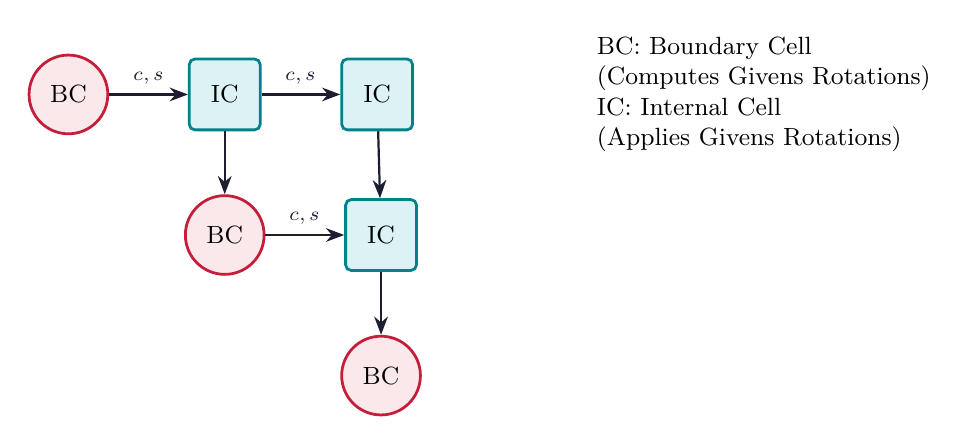
\begin{tikzpicture}[node distance=1.2cm and 1.2cm, every node/.style={font=\small}]
  % Boundary cell (circle)
  \node[circle, draw=myred, fill=hdrred, minimum size=1.0cm, line width=1.0pt] (bc1) at (0,0) {BC};
  
  % Internal cells (squares)
  \node[rectangle, draw=myteal, fill=hdrteal, minimum size=0.9cm, right=1.0cm of bc1, rounded corners=2pt, line width=1.0pt] (ic1) {IC};
  \node[rectangle, draw=myteal, fill=hdrteal, minimum size=0.9cm, right=1.0cm of ic1, rounded corners=2pt, line width=1.0pt] (ic2) {IC};
  
  \node[circle, draw=myred, fill=hdrred, minimum size=1.0cm, below=0.8cm of ic1, line width=1.0pt] (bc2) {BC};
  \node[rectangle, draw=myteal, fill=hdrteal, minimum size=0.9cm, right=1.0cm of bc2, rounded corners=2pt, line width=1.0pt] (ic3) {IC};
  
  \node[circle, draw=myred, fill=hdrred, minimum size=1.0cm, below=0.8cm of ic3, line width=1.0pt] (bc3) {BC};
  
  % Connections
  \draw[arrow] (bc1) -- node[above, font=\scriptsize] {$c, s$} (ic1);
  \draw[arrow] (ic1) -- node[above, font=\scriptsize] {$c, s$} (ic2);
  
  \draw[arrow] (bc2) -- node[above, font=\scriptsize] {$c, s$} (ic3);
  
  \draw[arrow] (ic1) -- (bc2);
  \draw[arrow] (ic2) -- (ic3);
  \draw[arrow] (ic3) -- (bc3);
  
  % Legend labels
  \node[right=2.2cm of ic2, align=left] {BC: Boundary Cell \\ (Computes Givens Rotations) \\ IC: Internal Cell \\ (Applies Givens Rotations)};
\end{tikzpicture}
\end{tcolorbox}

\begin{tcolorbox}[examplebox, title={Example: RLS Iteration Computation}]
Given $\lambda = 1.0$, the current estimate $\mathbf{w}(n-1) = [0.5, -0.2]^T$, and the inverse correlation matrix:
\[
  \mathbf{P}(n-1) = \begin{bmatrix} 2.0 & 0.5 \\ 0.5 & 1.0 \end{bmatrix}
\]
The new input sample vector is $\mathbf{x}(n) = [1.0, 2.0]^T$, and the desired signal is $d(n) = 0.8$. Execute one step of the RLS recursion to find the updated weight vector $\mathbf{w}(n)$.

\textbf{Solution:}
\begin{enumerate}[label=\textbf{\arabic*.}, leftmargin=*, itemsep=4pt]
  \item Compute the numerator of the gain vector:
    \[
      \mathbf{P}(n-1)\mathbf{x}(n) = \begin{bmatrix} 2.0 & 0.5 \\ 0.5 & 1.0 \end{bmatrix} \begin{bmatrix} 1.0 \\ 2.0 \end{bmatrix} = \begin{bmatrix} (2 \times 1) + (0.5 \times 2) \\ (0.5 \times 1) + (1 \times 2) \end{bmatrix} = \begin{bmatrix} 3.0 \\ 2.5 \end{bmatrix}
    \]
  \item Compute the denominator of the gain vector:
    \[
      \lambda + \mathbf{x}^T(n)\mathbf{P}(n-1)\mathbf{x}(n) = 1.0 + \begin{bmatrix} 1.0 & 2.0 \end{bmatrix} \begin{bmatrix} 3.0 \\ 2.5 \end{bmatrix} = 1.0 + (3.0 + 5.0) = 9.0
    \]
  \item Compute the gain vector $\mathbf{k}(n)$:
    \[
      \mathbf{k}(n) = \frac{1}{9.0} \begin{bmatrix} 3.0 \\ 2.5 \end{bmatrix} = \begin{bmatrix} 1/3 \\ 5/18 \end{bmatrix} \approx \begin{bmatrix} 0.3333 \\ 0.2778 \end{bmatrix}
    \]
  \item Compute the a priori estimation error $\xi(n)$:
    \[
      \xi(n) = d(n) - \mathbf{w}^T(n-1)\mathbf{x}(n) = 0.8 - \begin{bmatrix} 0.5 & -0.2 \end{bmatrix} \begin{bmatrix} 1.0 \\ 2.0 \end{bmatrix} = 0.8 - (0.5 - 0.4) = 0.7
    \]
  \item Update the weight vector $\mathbf{w}(n)$:
    \[
      \mathbf{w}(n) = \mathbf{w}(n-1) + \mathbf{k}(n)\xi(n) = \begin{bmatrix} 0.5 \\ -0.2 \end{bmatrix} + 0.7 \begin{bmatrix} 1/3 \\ 5/18 \end{bmatrix} = \begin{bmatrix} 0.5 + 0.2333 \\ -0.2 + 0.1944 \end{bmatrix} = \begin{bmatrix} 0.7333 \\ -0.0056 \end{bmatrix}
    \]
\end{enumerate}
\end{tcolorbox}

% ===============================================================================
% MANDATORY QUICK REVISION PAGE
% ===============================================================================
\newpage
\begin{center}
  {\large\bfseries\color{myred} Quick Revision --- Module V}\\[3pt]
  {\small\color{mydark} Recursive Least Squares (RLS) \& Advanced Topics $|$ PE-EC702A}
\end{center}
\noindent{\color{myred}\rule{\linewidth}{1.2pt}}
\vspace{4pt}

\begin{tcolorbox}[formulabox, title={\textbf{Key Formulas at a Glance}}]
\renewcommand{\arraystretch}{1.3}
\begin{tabularx}{\linewidth}{B{4.5cm} X}
RLS Cost Function & $\mathcal{E}(n) = \sum_{i=1}^n \lambda^{n-i} |e(i, n)|^2$ \\[6pt]
Correlation Matrix Update & $\mathbf{\Phi}(n) = \lambda \mathbf{\Phi}(n-1) + \mathbf{x}(n)\mathbf{x}^H(n)$ \\[6pt]
Matrix Inversion Lemma & $(\mathbf{A} + \mathbf{B}\mathbf{C}\mathbf{D})^{-1} = \mathbf{A}^{-1} - \mathbf{A}^{-1}\mathbf{B}(\mathbf{C}^{-1} + \mathbf{D}\mathbf{A}^{-1}\mathbf{B})^{-1}\mathbf{D}\mathbf{A}^{-1}$ \\[6pt]
Gain Vector $\mathbf{k}(n)$ & $\mathbf{k}(n) = \frac{\mathbf{P}(n-1)\mathbf{x}(n)}{\lambda + \mathbf{x}^H(n)\mathbf{P}(n-1)\mathbf{x}(n)}$ \\[6pt]
Weight Update & $\mathbf{w}(n) = \mathbf{w}(n-1) + \mathbf{k}(n)\xi^*(n)$ \quad ($\xi(n) = d(n) - \mathbf{w}^H(n-1)\mathbf{x}(n)$) \\[6pt]
Inverse Matrix Update & $\mathbf{P}(n) = \lambda^{-1} \left[ \mathbf{P}(n-1) - \mathbf{k}(n)\mathbf{x}^H(n)\mathbf{P}(n-1) \right]$
\end{tabularx}
\end{tcolorbox}

\begin{tcolorbox}[defbox, title={\textbf{One-Line Definitions}}]
\begin{itemize}[leftmargin=*, itemsep=2.5pt, topsep=0pt]
  \item \textbf{RLS Algorithm:} An adaptive filter algorithm that recursively finds coefficients to minimize deterministic sum of squared errors.
  \item \textbf{Forgetting Factor:} A scalar parameter $\lambda \le 1.0$ weighting recent data samples more heavily than older ones.
  \item \textbf{Gain Vector:} The vector $\mathbf{k}(n)$ that scales the error term in the RLS weight update equation.
  \item \textbf{Matrix Inversion Lemma:} A mathematical formula allowing recursive computation of matrix inverses without direct inversion.
  \item \textbf{Systolic Array:} A network of processing elements configured to execute parallel QRD matrix operations in hardware.
  \item \textbf{Boundary Cell:} A processor in a QRD systolic array calculating Givens rotation parameters (cosines and sines).
\end{itemize}
\end{tcolorbox}

\begin{tcolorbox}[exambox, title={\textbf{Frequently Asked / Viva Questions}}]
\begin{enumerate}[topsep=0pt, label=\textbf{Q\arabic*.}, itemsep=5pt]
  \item \Q{Compare RLS and LMS in terms of convergence speed and computational complexity.}
    RLS converges much faster than LMS (typically within $2M$ iterations, independent of eigenvalue spread) but requires higher computational complexity ($O(M^2)$ multiplications per sample compared to $O(M)$ for LMS).
  \item \Q{Explain the role of the forgetting factor $\lambda$ in the RLS cost function.}
    $\lambda$ determines the memory of the filter. If $\lambda = 1.0$, the filter has infinite memory (all data weighted equally). If $\lambda < 1.0$ (typically $0.98$), older data is exponentially attenuated, allowing the filter to track non-stationary changes.
  \item \Q{Write down the Woodbury identity (Matrix Inversion Lemma) and explain its use in RLS.}
    $(\mathbf{A} + \mathbf{U}\mathbf{C}\mathbf{V})^{-1} = \mathbf{A}^{-1} - \mathbf{A}^{-1}\mathbf{U}(\mathbf{C}^{-1} + \mathbf{V}\mathbf{A}^{-1}\mathbf{U})^{-1}\mathbf{V}\mathbf{A}^{-1}$. It is used to recursively update the inverse correlation matrix $\mathbf{P}(n) = \mathbf{\Phi}^{-1}(n)$ without performing an $O(M^3)$ matrix inversion step.
  \item \Q{What are the typical initialization values for the RLS algorithm?}
    $\mathbf{w}(0) = \mathbf{0}$ and $\mathbf{P}(0) = \delta^{-1}\mathbf{I}$, where $\delta$ is a small positive regularization parameter (e.g., $0.01$).
  \item \Q{What is the difference between a priori error $\xi(n)$ and a posteriori error $e(n)$ in RLS?}
    The a priori error $\xi(n) = d(n) - \mathbf{w}^H(n-1)\mathbf{x}(n)$ is calculated using the old weight vector, while the a posteriori error $e(n) = d(n) - \mathbf{w}^H(n)\mathbf{x}(n)$ is calculated using the updated weight vector.
  \item \Q{What is the purpose of using QR Decomposition (QRD) in RLS filters?}
    Standard RLS suffers from numerical instability under finite precision arithmetic, causing $\mathbf{P}(n)$ to lose positive-definiteness. QRD solves this by applying unitary rotations to the data matrix, ensuring numerical stability.
  \item \Q{What is the Affine Projection Algorithm (APA)?}
    APA is an intermediate algorithm between NLMS and RLS that updates weights based on the current and $P-1$ past input vectors, speeding up convergence for correlated signals with moderate complexity.
  \item \Q{What are partial update algorithms and where are they useful?}
    They are algorithms that update only a fraction of the filter weights at each time index to reduce power consumption and processing requirements, useful in acoustic echo cancellation in mobile phones.
  \item \Q{What are the functions of boundary cells and internal cells in a systolic array?}
    Boundary cells compute the Givens rotation parameters (cosine $c$ and sine $s$) to zero out elements of the incoming data matrix, while internal cells apply these rotations to the rest of the matrix rows.
  \item \Q{Why does RLS converge independently of the eigenvalue spread of the input signal?}
    Because RLS pre-whitens the input signal by multiplying the error vector with the inverse correlation matrix $\mathbf{P}(n)$, which de-correlates the input modes.
\end{enumerate}
\end{tcolorbox}

\begin{tcolorbox}[tikzbox, title={Comparison of LMS vs. RLS Algorithms}]
\renewcommand{\arraystretch}{1.45}
\par\noindent
\begin{tabularx}{\linewidth}{|B{3.2cm}|Y|Y|}
\hline
\rowcolor{hdrgray}
\textbf{Parameter} & \textbf{LMS Algorithm} & \textbf{RLS Algorithm} \\
\hline
\textbf{Convergence Rate} & Slow (dependent on input eigenvalue spread) & Fast (typically within $2M$ iterations, independent of spread) \\
\hline
\textbf{Complexity} & $O(M)$ multiplications per sample & $O(M^2)$ multiplications per sample \\
\hline
\textbf{Stability} & Stable if $0 < \mu < 2/\text{Tr}(\mathbf{R})$ & Can suffer from numerical instability in finite precision \\
\hline
\textbf{Parameters} & Step-size $\mu$ & Forgetting factor $\lambda$, regularization $\delta$ \\
\hline
\end{tabularx}
\end{tcolorbox}

\end{document}
